
\documentclass{article}
\usepackage[left=1cm,right=1cm]{geometry}
\usepackage{float}

\usepackage[htt]{hyphenat}
\usepackage{graphicx}
\usepackage{courier}



\begin{document}

\title{Atomic oven testing guide}
\date{\today}

\maketitle

\section{Wiring}

\begin{figure}[H]
    \center
    \includegraphics[scale=1]{figures/baseflange_wiring.pdf} 
    \caption{Wiring of in vacuum oven connector}
    \label{fig:baseflange_wiring}
\end{figure}

\section{Temperature readout}
Run the script in \texttt{oven\_test\_scripts/temperature\_readout} to print out temperature measurements in real time. Touch the thermocouples on each tube one after the other to check that the temperature reading changes.

\clearpage
\section{Low power testing}
Measure the current, voltage, and temperature characteristics of the oven at a low/safe power. Run the script in \texttt{oven\_test\_scripts/low\_power\_heating} and enter the channel of oven to be tested. Use the plotter script to make the graph, and the output should look like figure \ref{fig:low_power_heating}.
This measurement determines that everything is connected correctly, the restance of the oven and wiring, and the polarity of the thermocouple connection.

\begin{figure}
    \center
    \includegraphics[scale=1]{figures/current_vs_duty_0.pdf} 
    \caption{Example data for low\_power\_heating test. NB if the temperature reading decreases throughout the measurement, this indicates that the sensor polarity is inverted}
    \label{fig:low_power_heating}
\end{figure}

To invert the sensor polarity, run the script \texttt{calibration\_settings/reverse\_tc\_polarity.py} on the channel in question. This will save this configuration in firmware.

\clearpage
\section{Duty impulse response}

This measurement allows us to determine the temperature-current (T-C) cross-coupling of the oven.
This effect occurs when oven current flows through the thermocouple wiring in the vicinity of the spot weld.
Figures \ref{fig:duty_impulse_response_low} and \ref{fig:duty_impulse_response_high} show this measurement when there is a low and high T-C coefficient respectively.

\begin{figure}
    \center
    \includegraphics[scale=1]{figures/duty_impulse_response_data_0.pdf} 
    \caption{Example data for "duty impulse response" test where there is a low T-C coefficient.}
    \label{fig:duty_impulse_response_low}
\end{figure}

\begin{figure}
    \center
    \includegraphics[scale=1]{figures/duty_impulse_response_data_1.pdf} 
    \caption{Example data for "duty impulse response" test where there is a high T-C coefficient.}
    \label{fig:duty_impulse_response_high}
\end{figure}

Once the coupling coefficient is measured, it can be saved in the flash calibration for the microcontroller with the script \texttt{calibration\_settings/set\_tc\_current\_compensation.py}. To confirm that the compensation works, the duty impulse response script can be run again and the measurement should give a much lower coupling value.



\end{document}

